% !TEX encoding = UTF-8 Unicode 

\level{1}{Resoconto delle varie attività di verifica - Fase PD} 
	Sono riportati in questa appendice tutti i risultati ottenuti nei momenti di verifica, stabiliti nel \insdoc{Piano di Progetto v7.00} secondo la strategia di misurazione per il perseguimento della qualità individuata nel presente documento.\\
	Gli esiti sono presentati seguendo una precisa struttura. In particolare, essi sono suddivisi in base all'obiettivo e alla metrica che riguardano. Infatti, grazie ad essi il \insrole{Project Manager} deve essere in grado di capire quanto si è vicini al raggiungimento di un certo obiettivo prefissato.\\
	Per una descrizione dettagliata degli obiettivi si faccia riferimento alla sezione \nameref{sec:obiettivi}.

	\level{2}{Verifica dei prodotti}
		In questa sezione vengono riportati gli esiti delle attività di verifica svolte sui prodotti. Tale sezione è suddivisa ulteriormente in due, sulla base delle due tipologie di prodotti revisionati (documenti e software).
		\level{3}{Documenti}
			In questa sezione vengono riportati gli esiti delle attività di verifica svolte sui documenti. Tali esiti sono strettamente correlati con gli obiettivi di qualità dei documenti enunciati nel presente documento. Gli esiti sono utili al \insrole{Responsabile di Progetto} per modificare la strategia adottata e la pianificazione futura.
			\level{4}{Leggibilità e comprensibilità}
				Ci siamo imposti come obiettivo il fatto che i documenti siano leggibili e comprensibili da persone con un'educazione media. Per calcolare quanto si è vicini a tale obiettivo è stato scelto di fare uso dell'indice Gulpease.\\
				Durante questa fase si è preferito non perdere tempo nel calcolo di tale indice. Infatti, già da varie fasi i risultati si sono stabilizzati. È già stato raggiunto e largamente superato l'obiettivo \textbf{ottimale} che ci eravamo posti (valori maggiori di 50 per tutti i documenti).\\
			\level{4}{Correttezza ortografica}
				Ci siamo imposti come obiettivo il fatto che i documenti siano corretti dal punto di vista ortografico. Per calcolare quanto si è vicini a tale obiettivo è stato scelto di fare uso della seguente metrica: percentuale di errori ortografici rinvenuti in modo automatico e non corretti.\\
				Durante questa fase sono stati utilizzati strumenti automatici per la rilevazione di errori ortografici all'interno dei vari documenti. Si è inoltre tenuto conto di alcuni errori segnalati durante la Revisione di Qualifica.\\
				Si riporta di seguito la quantità degli errori rilevati per ciascuna tipologia durante l'intera fase:
				\begin{table}[H]
					\centering
						\begin{tabu}{| l | c |} \hline
							Ortografia errata (inglese) & 28\\ \hline
							Ortografia errata (italiano) & 5 \\ \hline
						\end{tabu}
					\caption{Errori ortografici trovati tramite verifica automatica dei documenti durante la Fase PD}
				\end{table}
				I pochi errori rinvenuti sono sintomo sia di una maggiore attenzione da parte dei membri del gruppo sia del fatto che durante questa fase la scrittura della documentazione non era preponderante.\\
				Tutti gli errori rinvenuti sono stati corretti manualmente. Dunque si ha raggiunto l'obiettivo considerato \textbf{ottimale} (nessun errore ortografico non corretto).
			\level{4}{Correttezza concettuale}
				Ci siamo imposti come obiettivo il fatto che i documenti siano corretti dal punto di vista concettuale. Per calcolare quanto si è vicini a tale obiettivo è stato scelto di fare uso della seguente metrica: percentuale di errori concettuali rinvenuti e non corretti.\\
				Per rilevare gli errori ci si è basati sulle osservazioni che ci sono state fatte in sede di Revisione di Qualifica. Inoltre, i \insrole{Verificatori} hanno provveduto a revisionare in modo approfondito i documenti, rilevando inesattezze, che poi sono state discusse e confermate dal gruppo.\\
				Si riporta in seguito la quantità di errori rilevati durante l'intera fase:
				\begin{table}[H]
					\centering
						\begin{tabu}{| l | c |} \hline
							Errori concettuali & 11\\ \hline
						\end{tabu}
					\caption{Errori concettuali trovati tramite verifica dei documenti durante la Fase PD}
				\end{table}
				Tutti gli errori rinvenuti sono stati discussi internamente al gruppo e tramite un incontro al quale ha partecipato il committente. La discussione ha sempre portato a una soluzione. La soluzione trovata è stata applicata ove fosse necessario. Dunque tutti gli errori rinvenuti sono stati sistemati e corretti. È stato dunque raggiunto l'obiettivo \textbf{ottimale} (nessun errore concettuale rinvenuto ma non sistemato).
		\level{3}{Codice e software}
			In questa sezione vengono riportati gli esiti delle attività di verifica svolte sul codice e sui prodotti software che si stanno implementando durante il progetto (Norris, Chuck e applicazione Android). Tali esiti sono strettamente correlati con gli obiettivi di qualità del software enunciati nel presente documento. Gli esiti sono utili al \insrole{Responsabile di Progetto} per modificare la strategia adottata e la pianificazione futura.
			\level{4}{Funzionalità}
				Il \groupname si è posto l'obiettivo di sviluppare software che disponga di tutte le funzionalità richieste dall'utente. Per calcolare quanto si è vicini a tale obiettivo è stato scelto di fare uso della seguente metrica: numero di requisiti funzionali realizzati.\\
				I requisiti funzionali sono di tre tipi:
				\begin{itemize}
					\item obbligatori;
					\item desiderabili;
					\item opzionali.
				\end{itemize}
				Viene qui presentato un riassunto dei dati riguardanti il numero di requisiti funzionali realizzati. Sulla base di questo si possono trarre conclusioni riguardanti l'obiettivo che ci siamo posti.
				\begin{table}[H]
					\centering
					\begin{tabu}{| l | c | c |}
						\hline
						Tipologia requisito   & Percentuale requisiti soddisfatti \\ \hline \hline
						Obbligatori           & 100\% \\ \hline
						Desiderabili          & 100\% \\ \hline
						Opzionali             & 98\% \\ \hline
					\end{tabu}
					\caption{Percentuali di requisiti funzionali realizzati in seguito alla fase PD}
				\end{table}
				Si può notare come sia stato raggiunto l'obiettivo \textbf{ottimale}. Infatti ci si augurava inizialmente di realizzare tutti i requisiti obbligatori e desiderabili e almeno il 95\% di quelli opzionali.
			\level{4}{Semplicità d'uso}
				Il \groupname si è posto l'obiettivo di sviluppare software che sia facilmente utilizzabile, in modo tale da favorirne l'apprendimento e la diffusione. Per calcolare quanto si è vicini a tale obiettivo è stato scelto di fare uso della seguente metrica: numero di parametri necessari in un metodo a disposizione dell'utente finale.\\
				Nell'applicazione Android l'utente non ha accesso a metodi, in quanto comunica con essa tramite interfaccia grafica. Neanche in Chuck possiamo affermare che l'utente ha accesso a metodi: egli deve solo utilizzare un singolo comando per creare un widget. Ha senso calcolare questa metrica solo in Norris, dove l'utente deve effettivamente invocare dei metodi per poter sfruttare le potenzialità del prodotto.\\
				Di seguito vengono presentati i risultati ottenuti durante le misurazioni. Si noti come non si tenga conto di tutti i metodi di tutte le classi di Norris, ma solo di quei metodi ai quali l'utente può accedere (i metodi che costituiscono le API del prodotto).\\
				\begin{table}[H]
					\centering
					\begin{tabu}{| l | c | c |}
						\hline
						Percentuale di metodi con più di 4 parametri   & 0\% \\ \hline
						Percentuale di metodi con 3 o 4 parametri      & 0\% \\ \hline
						Percentuale di metodi con 0, 1 o 2 parametri   & 100\% \\ \hline
					\end{tabu}
					\caption{Numero di parametri nei metodi a disposizione dell'utente in seguito alla fase PD}
				\end{table}
				Come si può notare tutte le API a disposizione dell'utente necessitano di un numero minore o uguale a due di parametri. Poichè ci eravamo posti come obiettivo minimo di avere solo metodi con 3-4 parametri e come obiettivo ottimale quello di avere solo metodi con un numero di parametri minore o uguale a due possiamo dire di aver raggiunto un esito \textbf{ottimale}.
			\level{4}{Manutenibilità e comprensibilità del codice}
				Il \groupname si è posto l'obiettivo di sviluppare software che sia facilmente manutenibile e comprensibile. Per calcolare quanto si è vicini a tale obiettivo è stato scelto di fare uso delle seguenti metriche:
				\begin{itemize}
					\item numero di statement di un metodo;
					\item numero di campi dati di una classe;
					\item grado di accoppiamento.
				\end{itemize}
				



				Nelle seguenti sezioni vengono riportate le percentuali precise di requisiti che sono stati soddisfatti (in base al prodotto e alle componenti che riguardano). In particolare per ogni prodotto e per ogni sua componente viene detto quanti requisiti funzionali obbligatori, desiderabili e opzionali sono stati realizzati. I dati sono stati ottenuti facilmente a partire dal tracciamento (componenti-requisiti) presente nel nostro tracker.

				\level{5}{Numero di requisiti funzionali obbligatori realizzati}
					Si riportano di seguito le percentuali di requisiti funzionali obbligatori realizzati dalle componenti di Norris.
					\begin{table}[H]
						\centering
							\begin{tabu}{| l | c | c |}
								\hline
								Componente	& Percentuale requisiti funzionali obbligatori soddisfatti	& Esito		\\ \hline \hline
								InternalAPIManager	& 100\% 	& Ottimale  \\ \hline
								ExternalAPIManager  & 	100\%	& Ottimale  \\ \hline
								DataModel  & 	100\%	& Ottimale  \\ \hline
							\end{tabu}
						\caption{Esiti del calcolo delle percentuali di requisiti funzionali obbligatori realizzati da Norris durante la Fase PD}
					\end{table}
					Come è possibile notare dalla tabella, la percentuale dei requisiti funzionali obbligatori soddisfatti da Norris ha raggiunto un esito complessivamente \textbf{ottimale}.\\
					Si riportano di seguito le percentuali di requisiti funzionali obbligatori realizzati dalle componenti di Chuck.
					\begin{table}[H]
						\centering
							\begin{tabu}{| l | c | c |}
								\hline
								Componente	& Percentuale requisiti funzionali obbligatori soddisfatti	& Esito		\\ \hline \hline
								Directive  &	100\% 	& Ottimale  \\ \hline
								ChartView  & 	100\%	& Ottimale  \\ \hline
								ViewModel  & 	100\%	& Ottimale  \\ \hline
								DataModel  & 	100\%	& Ottimale  \\ \hline
							\end{tabu}
						\caption{Esiti del calcolo delle percentuali di requisiti funzionali obbligatori realizzati da Chuck durante la Fase PD}
					\end{table}
					Come è possibile notare dalla tabella, la percentuale dei requisiti funzionali obbligatori soddisfatti da Chuck ha raggiunto un esito complessivamente \textbf{ottimale}.\\
					Si riportano di seguito le percentuali di requisiti funzionali obbligatori realizzati dalle componenti dell'Applicazione.
					\begin{table}[H]
						\centering
							\begin{tabu}{| l | c | c |}
								\hline
								Componente	& Percentuale requisiti funzionali obbligatori soddisfatti	& Esito		\\ \hline \hline
								Model				&   100\% 	& Ottimale \\ \hline
								Model:NorrisChart	&   100\% 	& Ottimale  \\ \hline
								Model:Service 		& 	100\%	& Ottimale   \\ \hline
								Presenter  			& 	100\%	& Ottimale  \\ \hline
								View  				& 	100\%	& Ottimale  \\ \hline
							\end{tabu}
						\caption{Esiti del calcolo delle percentuali di requisiti funzionali obbligatori realizzati dell'Applicazione durante la Fase PD}
					\end{table}
					Come è possibile notare dalla tabella la percentuale dei requisiti funzionali obbligatori soddisfatti dell'Applicazione ha raggiunto un esito \textbf{ottimale}.

				\level{5}{Numero di requisiti desiderabili funzionali realizzati}
					Si riportano di seguito le percentuali di requisiti desiderabili funzionali realizzati dalle componenti di Norris.
					\begin{table}[H]
						\centering
							\begin{tabu}{| l | c | c |}
								\hline
								Componente			& 	Percentuale requisiti funzionali desiderabili soddisfatti	& Esito		\\ \hline \hline
								InternalAPIManager	& 	100\% 	& Ottimale  \\ \hline
								ExternalAPIManager  & 	100\%	& Ottimale  \\ \hline
								DataModel  			& 	100\%	& Ottimale  \\ \hline
							\end{tabu}
						\caption{Esiti del calcolo delle percentuali di requisiti desiderabili funzionali realizzati da Norris durante la Fase PD}
					\end{table}
					Come è possibile notare dalla tabella la percentuale dei requisiti desiderabili funzionali soddisfatti da Norris ha raggiunto un esito \textbf{ottimale}. 
					\\ \\
					Si riportano di seguito le percentuali di requisiti desiderabili funzionali realizzati dalle componenti di Chuck.
					\begin{table}[H]
						\centering
							\begin{tabu}{| l | c | c |}
								\hline
								Componente	& Percentuale requisiti funzionali desiderabili soddisfatti	& Esito		\\ \hline \hline
								Directive	&	100\% 	& Ottimale  \\ \hline
								ChartView	& 	100\%	& Ottimale  \\ \hline
								ViewModel	& 	100\%	& Ottimale  \\ \hline
								DataModel	& 	100\%	& Ottimale  	\\ \hline
							\end{tabu}
						\caption{Esiti del calcolo delle percentuali di requisiti desiderabili funzionali realizzati da Chuck durante la Fase PD}
					\end{table}
					Come è possibile notare dalla tabella la percentuale dei requisiti desiderabili funzionali soddisfatti da Chuck ha raggiunto un esito, nel complesso, \textbf{ottimale}.

				\level{5}{Numero di requisiti opzionali funzionali realizzati}
				Si riportano di seguito le percentuali di requisiti opzionali funzionali realizzati dalle componenti di Norris.
				\begin{table}[H]
					\centering
						\begin{tabu}{| l | c | c |}
							\hline
							Componente	& Percentuale requisiti opzionali funzionali soddisfatti	& Esito		\\ \hline \hline
							InternalAPIManager	& 95\% 	& Accettabile  \\ \hline
							ExternalAPIManager  & 	96\%	& Accettabile  \\ \hline
							DataModel  & 	100\%	& Ottimale  \\ \hline
						\end{tabu}
					\caption{Esiti del calcolo delle percentuali di requisiti opzionali funzionali realizzati da Norris durante la Fase PD}
				\end{table}
				Complessivamente la percentuale dei requisiti funzionali opzionali realizzati in Norris è \textbf{ottimale}.\\				
				Si riportano di seguito le percentuali di requisiti opzionali funzionali realizzati dalle componenti di Chuck.
				\begin{table}[H]
					\centering
						\begin{tabu}{| l | c | c |}
							\hline
							Componente	& Numero requisiti opzionali funzionali soddisfatti	& Esito		\\ \hline \hline
							ViewModel  	& 90\%	& Accettabile  \\ \hline
							DataModel  	& 	97\%	& Accettabile  \\ \hline
						\end{tabu}
					\caption{Esiti del calcolo delle percentuali di requisiti opzionali funzionali realizzati da Chuck durante la Fase PD}
				\end{table}

			\level{4}{Percentuale di test di robustezza effettuati}
			Nella tabella seguente, vengono riportate le percentuali dei test effettuati sui tre prodotti: Norris, Chuck e applicazione Android.
			\begin{table}[H]
					\centering
						\begin{tabu}{| l | c | c |}
							\hline
							Prodotto	& Percentuale test superati	& Esito		\\ \hline \hline
							Norris	&	100\% 	& Ottimale  \\ \hline
							Chuck	& 	100\%	& Ottimale  \\ \hline
							Applicazione Android	& 	100\%	& Ottimale  \\ \hline
						\end{tabu}
					\caption{Esiti del calcolo delle percentuali dei test di robustezza superati durante la Fase PD}
				\end{table}
				
			\level{4}{Copertura del codice}
			Nella tabella seguente, vengono riportate le percentuali relative alla copertura del codice per le tre componenti del prodotto coi relativi esiti.
			\begin{table}[H]
					\centering
						\begin{tabu}{| l | c | c |}
							\hline
							Prodotto	& Percentuale codice testato	& Esito		\\ \hline \hline
							Norris	&	95\% 	& Ottimale  \\ \hline
							Chuck	& 	65\%	& Accettabile  \\ \hline
							Applicazione Android	& 	62\%	& Accettabile  \\ \hline
						\end{tabu}
					\caption{Esiti del calcolo delle percentuali della copertura del codice delle componenti durante la Fase PD}
				\end{table}
			\level{4}{Complessità ciclomatica, numero di statement per metodo e livello di annidamento}
			Per ogni metodo di ciascuna classe di Chuck e Norris, sono indicati, nella seguente tabella, i valori calcolati per le tre metriche: complessità ciclomatica (indicata con C.C.), numero di statement per metodo (indicato con N.S.) e livello di annidamento (indicato con L.A.).
				
				\begin{longtabu} spread 1cm [c]{|p{11cm}|p{1cm}|p{1cm}|p{1cm}|}
	\hline
					\rowfont{\bf \centering}
					Classe.metodo &
					C.C. &
					N.S.  &
					L.A. \\
					\hline
					\endhead
            
					\parbox[t]{4cm}{Chuck::Model::NorrisChart::BarChartInPlaceUpdater.update} &
                2 &
                18 &
                3\\\hline \parbox[t]{4cm}{Chuck::Model::NorrisChart::ChartImpl.createChart} &
                2 &
                5 &
                1\\\hline \parbox[t]{4cm}{Chuck::Model::NorrisChart::ChartImpl.getData} &
                1 &
                1 &
                0\\\hline \parbox[t]{4cm}{Chuck::Model::NorrisChart::ChartImpl.getId} &
                1 &
                1 &
                0\\\hline \parbox[t]{4cm}{Chuck::Model::NorrisChart::ChartImpl.getSettings} &
                1 &
                1 &
                0\\\hline \parbox[t]{4cm}{Chuck::Model::NorrisChart::ChartImpl.getType} &
                1 &
                1 &
                0\\\hline \parbox[t]{4cm}{Chuck::Model::NorrisChart::ChartImpl.setData} &
                1 &
                1 &
                0\\\hline \parbox[t]{4cm}{Chuck::Model::NorrisChart::ChartImpl.setSettings} &
                1 &
                4 &
                3\\\hline \parbox[t]{4cm}{Chuck::Model::NorrisChart::ChartImpl.update} &
                2 &
                7 &
                1\\\hline \parbox[t]{4cm}{Chuck::Model::NorrisChart::LineChartStreamUpdater.update} &
                4 &
                23 &
                6\\\hline \parbox[t]{4cm}{Chuck::Model::NorrisChart::LineChartInPlaceUpdater.update} &
                2 &
                18 &
                3\\\hline \parbox[t]{4cm}{Chuck::Model::NorrisChart::MapChartMovieUpdater.update} &
                1 &
                50 &
                6\\\hline \parbox[t]{4cm}{Chuck::Model::NorrisChart::MapChartInPlaceUpdater.update} &
                2 &
                19 &
                3\\\hline \parbox[t]{4cm}{Chuck::Model::NorrisChart::TableStreamUpdater.update} &
                6 &
                26 &
                5\\\hline \parbox[t]{4cm}{Chuck::Model::NorrisChart::TableInPlaceUpdater.update} &
                2 &
                19 &
                3\\\hline \parbox[t]{4cm}{Chuck::Model::Services::ChartRequester.bind} &
                1 &
                24 &
                1\\\hline \parbox[t]{4cm}{Chuck::ViewModel::BarChartViewModel.init} &
                1 &
                51 &
                2\\\hline \parbox[t]{4cm}{Chuck::ViewModel::BarChartViewModel.render} &
                1 &
                12 &
                2\\\hline \parbox[t]{4cm}{Chuck::ViewModel::LineChartViewModel.init} &
                1 &
                49 &
                2\\\hline \parbox[t]{4cm}{Chuck::ViewModel::LineChartViewModel.render} &
                1 &
                12 &
                1\\\hline \parbox[t]{4cm}{Chuck::ViewModel::MapChartViewModel.init} &
                1 &
                24 &
                1\\\hline \parbox[t]{4cm}{Chuck::ViewModel::MapChartViewModel.render} &
                1 &
                23 &
                2\\\hline \parbox[t]{4cm}{Chuck::ViewModel::TableViewModel.init} &
                1 &
                19 &
                1\\\hline \parbox[t]{4cm}{Chuck::ViewModel::TableViewModel.render} &
                1 &
                17 &
                2\\\hline \parbox[t]{4cm}{Norris::DataModel::NorrisChart::ChartImpl.getData} &
                1 &
                1 &
                0\\\hline \parbox[t]{4cm}{Norris::DataModel::NorrisChart::ChartImpl.getId} &
                1 &
                1 &
                0\\\hline \parbox[t]{4cm}{Norris::DataModel::NorrisChart::ChartImpl.getSettings} &
                1 &
                1 &
                0\\\hline \parbox[t]{4cm}{Norris::DataModel::NorrisChart::ChartImpl.getType} &
                1 &
                1 &
                0\\\hline \parbox[t]{4cm}{Norris::DataModel::NorrisChart::ChartImpl.setData} &
                1 &
                1 &
                0\\\hline \parbox[t]{4cm}{Norris::DataModel::NorrisChart::ChartImpl.setSettings} &
                2 &
                9 &
                4\\\hline \parbox[t]{4cm}{Norris::DataModel::NorrisChart::TableStreamUpdater.update} &
                6 &
                23 &
                6\\\hline \parbox[t]{4cm}{Norris::DataModel::NorrisChart::MapChartMovieUpdater.update} &
                5 &
                49 &
                5\\\hline \parbox[t]{4cm}{Norris::DataModel::NorrisChart::MapChartInPlaceUpdater.update} &
                3 &
                17 &
                3\\\hline \parbox[t]{4cm}{Norris::DataModel::NorrisChart::LineChartInStreamUpdater.update} &
                1 &
                1 &
                0\\\hline \parbox[t]{4cm}{Norris::DataModel::NorrisChart::LineChartInPlaceUpdater.update} &
                3 &
                16 &
                3\\\hline \parbox[t]{4cm}{Norris::DataModel::NorrisChart::ChartImpl.update} &
                2 &
                8 &
                1\\\hline \parbox[t]{4cm}{Norris::DataModel::NorrisChart::BarChartInPlaceUpdater.update} &
                1 &
                1 &
                0\\\hline \parbox[t]{4cm}{Norris::DataModel::NorrisChart::TableInPlaceUpdater.update} &
                3 &
                18 &
                3\\\hline \parbox[t]{4cm}{Norris::DataModel::NorrisImpl.createChart} &
                3 &
                8 &
                2\\\hline \parbox[t]{4cm}{Norris::DataModel::NorrisImpl.createPage} &
                2 &
                6 &
                1\\\hline \parbox[t]{4cm}{Norris::DataModel::NorrisImpl.getChart} &
                1 &
                1 &
                0\\\hline \parbox[t]{4cm}{Norris::DataModel::NorrisImpl.getCharts} &
                1 &
                1 &
                0\\\hline \parbox[t]{4cm}{Norris::DataModel::NorrisImpl.getPage} &
                1 &
                1 &
                0\\\hline \parbox[t]{4cm}{Norris::DataModel::NorrisImpl.getPages} &
                1 &
                1 &
                0\\\hline \parbox[t]{4cm}{Norris::DataModel::NorrisImpl.getSettings} &
                1 &
                1 &
                0\\\hline \parbox[t]{4cm}{Norris::DataModel::NorrisImpl.NorrisImpl} &
                2 &
                9 &
                1\\\hline \parbox[t]{4cm}{Norris::DataModel::NorrisImpl.setSettings} &
                1 &
                4 &
                3\\\hline \parbox[t]{4cm}{Norris::DataModel::NorrisPage::PageImpl.add} &
                4 &
                8 &
                2\\\hline \parbox[t]{4cm}{Norris::DataModel::NorrisPage::PageImpl.clearCharts} &
                1 &
                1 &
                0\\\hline \parbox[t]{4cm}{Norris::DataModel::NorrisPage::PageImpl.getCharts} &
                1 &
                1 &
                0\\\hline \parbox[t]{4cm}{Norris::DataModel::NorrisPage::PageImpl.getId} &
                1 &
                1 &
                0\\\hline \parbox[t]{4cm}{Norris::DataModel::NorrisPage::PageImpl.getSettings} &
                1 &
                1 &
                0\\\hline \parbox[t]{4cm}{Norris::DataModel::NorrisPage::PageImpl.setSettings} &
                1 &
                4 &
                3\\\hline \parbox[t]{4cm}{Norris::ExternalAPIManager::ChartRef.ChartRef} &
                2 &
                7 &
                1\\\hline \parbox[t]{4cm}{Norris::ExternalAPIManager::ChartRef.getData} &
                1 &
                1 &
                0\\\hline \parbox[t]{4cm}{Norris::ExternalAPIManager::ChartRef.getId} &
                1 &
                1 &
                0\\\hline \parbox[t]{4cm}{Norris::ExternalAPIManager::ChartRef.getSettings} &
                1 &
                1 &
                0\\\hline \parbox[t]{4cm}{Norris::ExternalAPIManager::ChartRef.getType} &
                1 &
                1 &
                0\\\hline \parbox[t]{4cm}{Norris::ExternalAPIManager::ExternalAPIConstructor.construct} &
                1 &
                3 &
                1\\\hline \parbox[t]{4cm}{Norris::ExternalAPIManager::ExternalAPIController.getChart} &
                1 &
                3 &
                0\\\hline \parbox[t]{4cm}{Norris::ExternalAPIManager::ExternalAPIController.getCharts} &
                1 &
                5 &
                1\\\hline \parbox[t]{4cm}{Norris::ExternalAPIManager::ExternalAPIConstructor.getInstance} &
                1 &
                1 &
                0\\\hline \parbox[t]{4cm}{Norris::ExternalAPIManager::ExternalAPIController.isLogged} &
                1 &
                3 &
                0\\\hline \parbox[t]{4cm}{Norris::ExternalAPIManager::ExternalAPIController.performKeepAlive} &
                1 &
                3 &
                0\\\hline \parbox[t]{4cm}{Norris::ExternalAPIManager::ExternalAPIController.performLogin} &
                1 &
                3 &
                0\\\hline \parbox[t]{4cm}{Norris::ExternalAPIManager::ExternalAPIController.performLogout} &
                1 &
                3 &
                0\\\hline \parbox[t]{4cm}{Norris::ExternalAPIManager::ExternalAPIConstructor.registerEndPoint} &
                1 &
                1 &
                0\\\hline \parbox[t]{4cm}{Norris::InternalAPIManager::ChartBridge.ChartBridge} &
                1 &
                2 &
                1\\\hline \parbox[t]{4cm}{Norris::InternalAPIManager::ChartBridge.getChartModel} &
                1 &
                1 &
                0\\\hline \parbox[t]{4cm}{Norris::InternalAPIManager::ChartBridge.getData} &
                1 &
                1 &
                0\\\hline \parbox[t]{4cm}{Norris::InternalAPIManager::ChartBridge.getId} &
                1 &
                1 &
                0\\\hline \parbox[t]{4cm}{Norris::InternalAPIManager::ChartBridge.getSettings} &
                1 &
                1 &
                0\\\hline \parbox[t]{4cm}{Norris::InternalAPIManager::ChartBridge.getType} &
                1 &
                1 &
                0\\\hline \parbox[t]{4cm}{Norris::InternalAPIManager::ChartBridge.setData} &
                1 &
                1 &
                0\\\hline \parbox[t]{4cm}{Norris::InternalAPIManager::ChartBridge.setSettings} &
                1 &
                1 &
                0\\\hline \parbox[t]{4cm}{Norris::InternalAPIManager::ChartBridge.update} &
                1 &
                1 &
                0\\\hline \parbox[t]{4cm}{Norris::InternalAPIManager::NorrisBridge.createChart} &
                1 &
                2 &
                0\\\hline \parbox[t]{4cm}{Norris::InternalAPIManager::NorrisBridge.createPage} &
                1 &
                2 &
                0\\\hline \parbox[t]{4cm}{Norris::InternalAPIManager::NorrisBridge.getChart} &
                1 &
                2 &
                0\\\hline \parbox[t]{4cm}{Norris::InternalAPIManager::NorrisBridge.getCharts} &
                1 &
                5 &
                0\\\hline \parbox[t]{4cm}{Norris::InternalAPIManager::NorrisBridge.getMiddleware} &
                1 &
                10 &
                1\\\hline \parbox[t]{4cm}{Norris::InternalAPIManager::NorrisBridge.getPage} &
                1 &
                2 &
                0\\\hline \parbox[t]{4cm}{Norris::InternalAPIManager::NorrisBridge.getPages} &
                1 &
                5 &
                0\\\hline \parbox[t]{4cm}{Norris::InternalAPIManager::NorrisBridge.getSettings} &
                1 &
                1 &
                0\\\hline \parbox[t]{4cm}{Norris::InternalAPIManager::NorrisBridge.setSettings} &
                1 &
                1 &
                0\\\hline \parbox[t]{4cm}{Norris::InternalAPIManager::PageBridge.add} &
                1 &
                3 &
                0\\\hline \parbox[t]{4cm}{Norris::InternalAPIManager::PageBridge.getCharts} &
                1 &
                5 &
                0\\\hline \parbox[t]{4cm}{Norris::InternalAPIManager::PageBridge.getId} &
                1 &
                1 &
                0\\\hline \parbox[t]{4cm}{Norris::InternalAPIManager::PageBridge.getSettings} &
                1 &
                1 &
                0\\\hline \parbox[t]{4cm}{Norris::InternalAPIManager::PageBridge.PageBridge} &
                1 &
                2 &
                1\\\hline \parbox[t]{4cm}{Norris::InternalAPIManager::PageBridge.setCharts} &
                1 &
                3 &
                0\\\hline \parbox[t]{4cm}{Norris::InternalAPIManager::PageBridge.setSettings} &
                1 &
                1 &
                0\\\hline                 \caption{Metodi e metriche Norris / Chuck}
				\end{longtabu}

			Per ogni metodo di ciascuna classe dell'applicazione Android, sono indicati, nella seguente tabella, i valori calcolati per le tre metriche: complessità ciclomatica (indicata con C.C.), numero di statement per metodo (indicato con N.S.) e livello di annidamento (indicato con L.A.).
				
\begin{longtabu} spread 1cm [c]{|p{11cm}|p{1cm}|p{1cm}|p{1cm}|}
					\hline
					\rowfont{\bf \centering}
					Classe.metodo &
					C.C. &
					N.S.  &
					L.A. 
					\\
					\hline
					\endhead
            
					\parbox[t]{4cm}{Applicazione::Model::NorrisChart::ChartImpl.create} &
                1 &
                4 &
                1\\\hline \parbox[t]{4cm}{Applicazione::Model::NorrisChart::TableCell.getBackgroundColor} &
                1 &
                1 &
                0\\\hline \parbox[t]{4cm}{Applicazione::Model::NorrisChart::MapChartSettingsImpl.getCamera-\\ZoomHeight} &
                1 &
                4 &
                1\\\hline \parbox[t]{4cm}{Applicazione::Model::NorrisChart::ChartImpl.getData} &
                1 &
                1 &
                0\\\hline \parbox[t]{4cm}{Applicazione::Model::NorrisChart::LineChartDataImpl.getData} &
                1 &
                1 &
                0\\\hline \parbox[t]{4cm}{Applicazione::Model::NorrisChart::BarChartDataImpl.getData} &
                1 &
                1 &
                0\\\hline \parbox[t]{4cm}{Applicazione::Model::NorrisChart::TableDataImpl.getData} &
                1 &
                1 &
                0\\\hline \parbox[t]{4cm}{Applicazione::Model::NorrisChart::MapChartDataImpl.getData} &
                1 &
                1 &
                0\\\hline \parbox[t]{4cm}{Applicazione::Model::NorrisChart::TableRow.getData} &
                1 &
                1 &
                0\\\hline \parbox[t]{4cm}{Applicazione::Model::NorrisChart::MapSet.getData} &
                1 &
                1 &
                0\\\hline \parbox[t]{4cm}{Applicazione::Model::NorrisChart::TableCell.getData} &
                1 &
                1 &
                0\\\hline \parbox[t]{4cm}{Applicazione::Model::NorrisChart::TableStreamUpdate.getData} &
                1 &
                1 &
                0\\\hline \parbox[t]{4cm}{Applicazione::Model::NorrisChart::TableInPlaceUpdate.getData} &
                1 &
                1 &
                0\\\hline \parbox[t]{4cm}{Applicazione::Model::NorrisChart::MapChartInPlaceUpdate.getData} &
                1 &
                1 &
                0\\\hline \parbox[t]{4cm}{Applicazione::Model::NorrisChart::TableCellInPlaceUpdate.getData} &
                1 &
                1 &
                0\\\hline \parbox[t]{4cm}{Applicazione::Model::NorrisChart::MapChartElementInPlace-\\Update.getData} &
                1 &
                1 &
                0\\\hline \parbox[t]{4cm}{Applicazione::Model::NorrisChart::MapChartStreamUpdate.getData} &
                1 &
                1 &
                0\\\hline \parbox[t]{4cm}{Applicazione::Model::NorrisChart::MapChartDeleteUpdate.getData} &
                1 &
                1 &
                0\\\hline \parbox[t]{4cm}{Applicazione::Model::NorrisChart::LineChartStreamUpdate.getData} &
                1 &
                1 &
                0\\\hline \parbox[t]{4cm}{Applicazione::Model::NorrisChart::LineChartElementStream-\\Update.getData} &
                1 &
                1 &
                0\\\hline \parbox[t]{4cm}{Applicazione::Model::NorrisChart::BarChartInPlaceUpdate.getData} &
                1 &
                1 &
                0\\\hline \parbox[t]{4cm}{Applicazione::Model::NorrisChart::BarChartElementInPlace-\\Update.getData} &
                1 &
                1 &
                0\\\hline \parbox[t]{4cm}{Applicazione::Model::NorrisChart::LineChartInPlaceUpdate.getData} &
                1 &
                1 &
                0\\\hline \parbox[t]{4cm}{Applicazione::Model::NorrisChart::LineChartElementInPlace-\\Updater.getData} &
                1 &
                1 &
                0\\\hline \parbox[t]{4cm}{Applicazione::Model::NorrisChart::MapChartMovieUpdate.getDeleteData} &
                1 &
                1 &
                0\\\hline \parbox[t]{4cm}{Applicazione::Model::NorrisChart::TableCell.getFontColor} &
                1 &
                1 &
                0\\\hline \parbox[t]{4cm}{Applicazione::Model::NorrisChart::LineChartSettingsImpl.getGrid-\\Visibility} &
                1 &
                4 &
                1\\\hline \parbox[t]{4cm}{Applicazione::Model::NorrisChart::BarChartSettingsImpl.getGrid-\\Visibility} &
                1 &
                4 &
                1\\\hline \parbox[t]{4cm}{Applicazione::Model::NorrisChart::ChartImpl.getId} &
                1 &
                1 &
                0\\\hline \parbox[t]{4cm}{Applicazione::Model::NorrisChart::MapPoint.getId} &
                1 &
                1 &
                0\\\hline \parbox[t]{4cm}{Applicazione::Model::NorrisChart::MapChartElementInPlace-\\Update.getId} &
                1 &
                1 &
                0\\\hline \parbox[t]{4cm}{Applicazione::Model::NorrisChart::MapChartElementInPlace-\\Update.getIndex} &
                1 &
                1 &
                0\\\hline \parbox[t]{4cm}{Applicazione::Model::NorrisChart::MapChartElementInPlace-\\Update.getIndex} &
                1 &
                1 &
                0\\\hline \parbox[t]{4cm}{Applicazione::Model::NorrisChart::MapChartMovieUpdate.get-\\InPlaceData} &
                1 &
                1 &
                0\\\hline \parbox[t]{4cm}{Applicazione::Model::NorrisChart::TableDataImpl.getLabel} &
                1 &
                1 &
                0\\\hline \parbox[t]{4cm}{Applicazione::Model::NorrisChart::LineChartElement-\\StreamUpdate.getLabel} &
                1 &
                1 &
                0\\\hline \parbox[t]{4cm}{Applicazione::Model::NorrisChart::MapPoint.getLatitude} &
                1 &
                1 &
                0\\\hline \parbox[t]{4cm}{Applicazione::Model::NorrisChart::LineChartSettingsImpl.get-\\LegendPosition} &
                1 &
                1 &
                0\\\hline \parbox[t]{4cm}{Applicazione::Model::NorrisChart::BarChartSettingsImpl.get-\\LegendPosition} &
                1 &
                1 &
                0\\\hline \parbox[t]{4cm}{Applicazione::Model::NorrisChart::MapPoint.getLongitude} &
                1 &
                1 &
                0\\\hline \parbox[t]{4cm}{Applicazione::Model::NorrisChart::BarChartSettingsImpl.getOrientation} &
                1 &
                4 &
                1\\\hline \parbox[t]{4cm}{Applicazione::Model::NorrisChart::ChartImpl.getSettings} &
                1 &
                1 &
                0\\\hline \parbox[t]{4cm}{Applicazione::Model::NorrisChart::MapChartMovieUpdate.getStream-\\Data} &
                1 &
                1 &
                0\\\hline \parbox[t]{4cm}{Applicazione::Model::NorrisChart::ChartImpl.getType} &
                1 &
                1 &
                0\\\hline \parbox[t]{4cm}{Applicazione::Model::NorrisChart::TableCellInPlaceUpdate.getX} &
                1 &
                1 &
                0\\\hline \parbox[t]{4cm}{Applicazione::Model::NorrisChart::BarChartElementInPlace-\\Update.getX} &
                1 &
                1 &
                0\\\hline \parbox[t]{4cm}{Applicazione::Model::NorrisChart::LineChartElementInPlace-\\Updater.getX} &
                1 &
                1 &
                0\\\hline \parbox[t]{4cm}{Applicazione::Model::NorrisChart::LineChartSettingsImpl.getX-\\AxisName} &
                1 &
                4 &
                1\\\hline \parbox[t]{4cm}{Applicazione::Model::NorrisChart::BarChartSettingsImpl.getXAxisName} &
                1 &
                4 &
                1\\\hline \parbox[t]{4cm}{Applicazione::Model::NorrisChart::MapChartSettingsImpl.getXCamera-\\Coordinate} &
                1 &
                4 &
                1\\\hline \parbox[t]{4cm}{Applicazione::Model::NorrisChart::TableCellInPlaceUpdate.getY} &
                1 &
                1 &
                0\\\hline \parbox[t]{4cm}{Applicazione::Model::NorrisChart::BarChartElementInPlaceUpdate.getY} &
                1 &
                1 &
                0\\\hline \parbox[t]{4cm}{Applicazione::Model::NorrisChart::LineChartElementInPlace-\\Updater.getY} &
                1 &
                1 &
                0\\\hline \parbox[t]{4cm}{Applicazione::Model::NorrisChart::LineChartSettingsImpl.getYAxisName} &
                1 &
                4 &
                1\\\hline \parbox[t]{4cm}{Applicazione::Model::NorrisChart::BarChartSettingsImpl.getYAxisName} &
                1 &
                4 &
                1\\\hline \parbox[t]{4cm}{Applicazione::Model::NorrisChart::MapChartSettingsImpl.getYCamera-\\Coordinate} &
                1 &
                4 &
                1\\\hline \parbox[t]{4cm}{Applicazione::Model::NorrisChart::TableCell.setBackgroundColor} &
                1 &
                1 &
                0\\\hline \parbox[t]{4cm}{Applicazione::Model::NorrisChart::ChartImpl.setData} &
                1 &
                1 &
                0\\\hline \parbox[t]{4cm}{Applicazione::Model::NorrisChart::LineChartDataImpl.setData} &
                1 &
                1 &
                0\\\hline \parbox[t]{4cm}{Applicazione::Model::NorrisChart::BarChartDataImpl.setData} &
                1 &
                1 &
                0\\\hline \parbox[t]{4cm}{Applicazione::Model::NorrisChart::TableDataImpl.setData} &
                1 &
                1 &
                0\\\hline \parbox[t]{4cm}{Applicazione::Model::NorrisChart::MapChartDataImpl.setData} &
                1 &
                1 &
                0\\\hline \parbox[t]{4cm}{Applicazione::Model::NorrisChart::TableRow.setData} &
                1 &
                1 &
                0\\\hline \parbox[t]{4cm}{Applicazione::Model::NorrisChart::MapSet.setData} &
                1 &
                1 &
                0\\\hline \parbox[t]{4cm}{Applicazione::Model::NorrisChart::TableCell.setData} &
                1 &
                1 &
                0\\\hline \parbox[t]{4cm}{Applicazione::Model::NorrisChart::TableCell.setFontColor} &
                1 &
                1 &
                0\\\hline \parbox[t]{4cm}{Applicazione::Model::NorrisChart::MapPoint.setLatitude} &
                1 &
                1 &
                0\\\hline \parbox[t]{4cm}{Applicazione::Model::NorrisChart::MapPoint.setLongitude} &
                1 &
                1 &
                0\\\hline \parbox[t]{4cm}{Applicazione::Model::NorrisChart::ChartImpl.setSettings} &
                1 &
                4 &
                3\\\hline \parbox[t]{4cm}{Applicazione::Model::NorrisChart::TableInPlaceUpdater.update} &
                1 &
                4 &
                1\\\hline \parbox[t]{4cm}{Applicazione::Model::NorrisChart::BarChartInPlaceUpdater.update} &
                1 &
                1 &
                0\\\hline \parbox[t]{4cm}{Applicazione::Model::NorrisChart::ChartImpl.update} &
                1 &
                4 &
                1\\\hline \parbox[t]{4cm}{Applicazione::Model::NorrisChart::LineChartInPlaceUpdater.update} &
                1 &
                4 &
                1\\\hline \parbox[t]{4cm}{Applicazione::Model::NorrisChart::LineChartStreamUpdater.update} &
                2 &
                13 &
                2\\\hline \parbox[t]{4cm}{Applicazione::Model::NorrisChart::MapChartMovieUpdater.update} &
                1 &
                28 &
                4\\\hline \parbox[t]{4cm}{Applicazione::Model::NorrisChart::MapChartInPlaceUpdater.update} &
                1 &
                4 &
                1\\\hline \parbox[t]{4cm}{Applicazione::Model::NorrisChart::TableStreamUpdater.update} &
                1 &
                8 &
                2\\\hline \parbox[t]{4cm}{Applicazione::Model::NorrisSessionInfoImpl.getAddress} &
                1 &
                1 &
                0\\\hline \parbox[t]{4cm}{Applicazione::Model::NorrisSessionInfoImpl.getAuthCookie} &
                1 &
                1 &
                0\\\hline \parbox[t]{4cm}{Applicazione::Model::NorrisSessionInfoImpl.getInstance} &
                2 &
                3 &
                1\\\hline \parbox[t]{4cm}{Applicazione::Model::NorrisSessionInfoImpl.isLogged} &
                1 &
                1 &
                0\\\hline \parbox[t]{4cm}{Applicazione::Model::NorrisSessionInfoImpl.login} &
                1 &
                1 &
                0\\\hline \parbox[t]{4cm}{Applicazione::Model::NorrisSessionInfoImpl.logout} &
                1 &
                1 &
                0\\\hline \parbox[t]{4cm}{Applicazione::Model::NorrisSessionInfoImpl.setAddress} &
                1 &
                1 &
                0\\\hline \parbox[t]{4cm}{Applicazione::Model::Service::ChartReceiverImpl.getChart} &
                1 &
                14 &
                1\\\hline \parbox[t]{4cm}{Applicazione::Model::Service::ChartReceiverImpl.getInstance} &
                1 &
                3 &
                1\\\hline \parbox[t]{4cm}{Applicazione::Model::Service::ChartReceiverImpl.startUpdateEvent} &
                1 &
                4 &
                0\\\hline \parbox[t]{4cm}{Applicazione::Model::Service::ChartReceiverImpl.stopUpdateEvent} &
                1 &
                2 &
                0\\\hline \parbox[t]{4cm}{Applicazione::Presenter::BarChartPresenterImpl.applySettings} &
                1 &
                10 &
                0\\\hline \parbox[t]{4cm}{Applicazione::Presenter::BarChartPresenterImpl.update} &
                2 &
                21 &
                3\\\hline \parbox[t]{4cm}{Applicazione::Presenter::HttpRequesterWithCookie.getList} &
                1 &
                11 &
                1\\\hline \parbox[t]{4cm}{Applicazione::Presenter::HttpRequesterWithCookie.login} &
                1 &
                27 &
                1\\\hline \parbox[t]{4cm}{Applicazione::Presenter::HttpRequesterWithCookie.logout} &
                2 &
                7 &
                1\\\hline \parbox[t]{4cm}{Applicazione::Presenter::JSONParser.getInstance} &
                1 &
                3 &
                0\\\hline \parbox[t]{4cm}{Applicazione::Presenter::JSONParser.parseBarChart} &
                1 &
                25 &
                2\\\hline \parbox[t]{4cm}{Applicazione::Presenter::JSONParser.parseBarChartInPlaceUpdate} &
                1 &
                10 &
                1\\\hline \parbox[t]{4cm}{Applicazione::Presenter::JSONParser.parseBarChartSettings} &
                1 &
                1 &
                0\\\hline \parbox[t]{4cm}{Applicazione::Presenter::JSONParser.parseLineChart} &
                1 &
                25 &
                2\\\hline \parbox[t]{4cm}{Applicazione::Presenter::JSONParser.parseLineChartInPlaceUpdate} &
                1 &
                10 &
                1\\\hline \parbox[t]{4cm}{Applicazione::Presenter::JSONParser.parseLineChartSettings} &
                1 &
                1 &
                0\\\hline \parbox[t]{4cm}{Applicazione::Presenter::JSONParser.parseLineChartStreamUpdate} &
                1 &
                11 &
                2\\\hline \parbox[t]{4cm}{Applicazione::Presenter::JSONParser.parseMapChart} &
                1 &
                35 &
                2\\\hline \parbox[t]{4cm}{Applicazione::Presenter::JSONParser.parseMapChartDeleteUpdate} &
                1 &
                13 &
                2\\\hline \parbox[t]{4cm}{Applicazione::Presenter::JSONParser.parseMapChartInPlaceUpdate} &
                1 &
                24 &
                2\\\hline \parbox[t]{4cm}{Applicazione::Presenter::JSONParser.parseMapChartMovieUpdate} &
                1 &
                15 &
                1\\\hline \parbox[t]{4cm}{Applicazione::Presenter::JSONParser.parseMapChartSettings} &
                1 &
                1 &
                0\\\hline \parbox[t]{4cm}{Applicazione::Presenter::JSONParser.parseMapChartStreamUpdate} &
                1 &
                12 &
                2\\\hline \parbox[t]{4cm}{Applicazione::Presenter::JSONParser.parseTable} &
                1 &
                23 &
                3\\\hline \parbox[t]{4cm}{Applicazione::Presenter::JSONParser.parseTableInPlaceUpdate} &
                1 &
                19 &
                2\\\hline \parbox[t]{4cm}{Applicazione::Presenter::JSONParser.parseTableSettings} &
                1 &
                1 &
                0\\\hline \parbox[t]{4cm}{Applicazione::Presenter::JSONParser.parseTableStreamUpdate} &
                1 &
                19 &
                3\\\hline \parbox[t]{4cm}{Applicazione::Presenter::LineChartPresenterImpl.applySettings} &
                1 &
                9 &
                0\\\hline \parbox[t]{4cm}{Applicazione::Presenter::LineChartPresenterImpl.update} &
                4 &
                30 &
                3\\\hline \parbox[t]{4cm}{Applicazione::Presenter::ListPresenterImpl.onItemClicked} &
                1 &
                1 &
                0\\\hline \parbox[t]{4cm}{Applicazione::Presenter::ListPresenterImpl.onLogoutClick} &
                1 &
                2 &
                0\\\hline \parbox[t]{4cm}{Applicazione::Presenter::ListPresenterImpl.onResume} &
                1 &
                6 &
                0\\\hline \parbox[t]{4cm}{Applicazione::Presenter::LoginPresenterImpl.onLoginClick} &
                2 &
                7 &
                1\\\hline \parbox[t]{4cm}{Applicazione::Presenter::MapChartPresenterImpl.applySettings} &
                1 &
                4 &
                0\\\hline \parbox[t]{4cm}{Applicazione::Presenter::MapChartPresenterImpl.update} &
                4 &
                28 &
                3\\\hline \parbox[t]{4cm}{Applicazione::Presenter::PresenterImpl.create} &
                1 &
                3 &
                0\\\hline \parbox[t]{4cm}{Applicazione::Presenter::PresenterImpl.registerFactory} &
                1 &
                1 &
                0\\\hline \parbox[t]{4cm}{Applicazione::Presenter::TablePresenterImpl.applySettings} &
                1 &
                3 &
                0\\\hline \parbox[t]{4cm}{Applicazione::Presenter::TablePresenterImpl.update} &
                4 &
                28 &
                3\\\hline \parbox[t]{4cm}{Applicazione::View::BarChartActivity.onCreate} &
                1 &
                4 &
                0\\\hline \parbox[t]{4cm}{Applicazione::View::BarChartActivity.onPause} &
                1 &
                4 &
                0\\\hline \parbox[t]{4cm}{Applicazione::View::BarChartActivity.onResume} &
                1 &
                4 &
                0\\\hline \parbox[t]{4cm}{Applicazione::View::BarChartActivity.renderChart} &
                1 &
                11 &
                3\\\hline \parbox[t]{4cm}{Applicazione::View::BarChartActivity.setAxisName} &
                2 &
                6 &
                1\\\hline \parbox[t]{4cm}{Applicazione::View::BarChartActivity.setBarDataSetSpacing} &
                1 &
                3 &
                0\\\hline \parbox[t]{4cm}{Applicazione::View::BarChartActivity.setBarValueSpacing} &
                1 &
                4 &
                1\\\hline \parbox[t]{4cm}{Applicazione::View::BarChartActivity.setLegendPosition} &
                1 &
                13 &
                1\\\hline \parbox[t]{4cm}{Applicazione::View::BarChartActivity.setOrientation} &
                2 &
                12 &
                1\\\hline \parbox[t]{4cm}{Applicazione::View::BarChartActivity.showGrid} &
                1 &
                4 &
                0\\\hline \parbox[t]{4cm}{Applicazione::View::ChartActivity.getChartId} &
                1 &
                1 &
                0\\\hline \parbox[t]{4cm}{Applicazione::View::ChartActivity.getId} &
                1 &
                1 &
                0\\\hline \parbox[t]{4cm}{Applicazione::View::ChartActivity.renderChart} &
                0 &
                0 &
                0\\\hline \parbox[t]{4cm}{Applicazione::View::ChartActivity.setChartTitle} &
                1 &
                1 &
                0\\\hline \parbox[t]{4cm}{Applicazione::View::ChartActivity.setDescription} &
                1 &
                1 &
                0\\\hline \parbox[t]{4cm}{Applicazione::View::LineChartActivity.onCreate} &
                1 &
                4 &
                0\\\hline \parbox[t]{4cm}{Applicazione::View::LineChartActivity.onPause} &
                1 &
                4 &
                0\\\hline \parbox[t]{4cm}{Applicazione::View::LineChartActivity.onResume} &
                1 &
                4 &
                0\\\hline \parbox[t]{4cm}{Applicazione::View::LineChartActivity.renderChart} &
                1 &
                19 &
                0\\\hline \parbox[t]{4cm}{Applicazione::View::LineChartActivity.setAxisName} &
                1 &
                2 &
                0\\\hline \parbox[t]{4cm}{Applicazione::View::LineChartActivity.setCubicLines} &
                1 &
                4 &
                1\\\hline \parbox[t]{4cm}{Applicazione::View::LineChartActivity.setDotRadius} &
                1 &
                8 &
                2\\\hline \parbox[t]{4cm}{Applicazione::View::LineChartActivity.setDottedLines} &
                1 &
                7 &
                2\\\hline \parbox[t]{4cm}{Applicazione::View::LineChartActivity.setLegendPosition} &
                1 &
                13 &
                1\\\hline \parbox[t]{4cm}{Applicazione::View::LineChartActivity.setSeriesColor} &
                1 &
                1 &
                0\\\hline \parbox[t]{4cm}{Applicazione::View::LineChartActivity.showGrid} &
                1 &
                4 &
                0\\\hline \parbox[t]{4cm}{Applicazione::View::ListActivity.navigate} &
                1 &
                3 &
                0\\\hline \parbox[t]{4cm}{Applicazione::View::ListActivity.navigateToLoginView} &
                1 &
                3 &
                0\\\hline \parbox[t]{4cm}{Applicazione::View::ListActivity.onCreate} &
                1 &
                5 &
                0\\\hline \parbox[t]{4cm}{Applicazione::View::ListActivity.onItemClick} &
                1 &
                1 &
                0\\\hline \parbox[t]{4cm}{Applicazione::View::ListActivity.onLogoutClick} &
                1 &
                1 &
                0\\\hline \parbox[t]{4cm}{Applicazione::View::ListActivity.renderList} &
                1 &
                26 &
                2\\\hline \parbox[t]{4cm}{Applicazione::View::ListActivity.showChartDetailView} &
                1 &
                11 &
                1\\\hline \parbox[t]{4cm}{Applicazione::View::LoginActivity.onCreate} &
                1 &
                5 &
                0\\\hline \parbox[t]{4cm}{Applicazione::View::LoginActivity.onLoginClick} &
                1 &
                1 &
                0\\\hline \parbox[t]{4cm}{Applicazione::View::LoginActivity.showAuthenticationError} &
                1 &
                1 &
                0\\\hline \parbox[t]{4cm}{Applicazione::View::LoginActivity.showListView} &
                1 &
                2 &
                0\\\hline \parbox[t]{4cm}{Applicazione::View::LoginActivity.showProgress} &
                2 &
                4 &
                0\\\hline \parbox[t]{4cm}{Applicazione::View::MapChartActivity.onCreate} &
                1 &
                4 &
                0\\\hline \parbox[t]{4cm}{Applicazione::View::MapChartActivity.onPause} &
                1 &
                2 &
                0\\\hline \parbox[t]{4cm}{Applicazione::View::MapChartActivity.onResume} &
                1 &
                3 &
                0\\\hline \parbox[t]{4cm}{Applicazione::View::MapChartActivity.renderChart} &
                1 &
                18 &
                3\\\hline \parbox[t]{4cm}{Applicazione::View::MapChartActivity.setCameraCoordinate} &
                1 &
                1 &
                0\\\hline \parbox[t]{4cm}{Applicazione::View::MapChartActivity.setCameraZoom} &
                1 &
                1 &
                0\\\hline \parbox[t]{4cm}{Applicazione::View::MapChartActivity.setUpMapIfNeeded} &
                1 &
                4 &
                2\\\hline \parbox[t]{4cm}{Applicazione::View::TableActivity.onCreate} &
                1 &
                3 &
                0\\\hline \parbox[t]{4cm}{Applicazione::View::TableActivity.onPause} &
                1 &
                2 &
                0\\\hline \parbox[t]{4cm}{Applicazione::View::TableActivity.onResume} &
                1 &
                3 &
                0\\\hline \parbox[t]{4cm}{Applicazione::View::TableActivity.renderChart} &
                1 &
                24 &
                3\\\hline \parbox[t]{4cm}{Applicazione::View::TableActivity.showCellBorderLine} &
                2 &
                4 &
                1\\\hline                 \caption{Metodi e metriche applicazione}
				\end{longtabu}

				
			\level{4}{Grado di accoppiamento dei componenti}
			Si riporta di seguito, per ogni componente,il grado di accoppiamento afferente ed efferente.
			\begin{table}[H]
				\centering
					\begin{tabu}{| l | c | c | c | c | c | c | }
						\hline
						Componente					& Afferente & Esiti Afferente & Efferente & Esiti Efferente 	\\ \hline \hline
						Norris::InternalAPIManager	& 1 & Ottimale & 3 & Ottimale  \\ \hline
						Norris::ExternalAPIManager  & 0 & Ottimale & 9 & Non Accettabile   \\ \hline
						Norris::DataModel  			& 4 & Ottimale & 3 & Ottimale   \\ \hline
						Chuck::Model 				& 2 & Ottimale & 4 & Ottimale   \\ \hline
						Chuck::ViewModel 			& 8 & Non Accettabile & 6 & Accettabile   \\ \hline
						Chuck::Directive 			& 0 & Ottimale & 12 & Non Accettabile   \\ \hline
						Chuck::View 				& 4 & Ottimale & 4 & Ottimale   \\ \hline
						App::Model 					& 4 & Ottimale & 2 & Ottimale   \\ \hline
						App::Presenter 				& 2 & Ottimale & 6 & Accettabile   \\ \hline
						App::View 					& 1 & Ottimale & 6 & Accettabile   \\ \hline
					\end{tabu}
				\caption{Esiti del calcolo del grado di accoppiamento per le componenti durante la Fase PD}
			\end{table}
			Come è possibile notare dalla tabella, abbiamo ottenuto buoni risultati sia per Norris sia per l'applicazione Android, mentre i valori del grado di accoppiamento afferente della componente ViewModel di Chuck sono risultati molto alti, in quanto rappresenta la componente principale di Chuck.
			 
	\level{2}{Verifica dei processi}
		\level{3}{Processo di documentazione}
			\level{4}{Livello CMM}
			In questa fase, il livello CMM del processo di documentazione si assesta al terzo gradino della scala CMM.

			\level{4}{Schedule Variance}
			La maggior parte delle attività pianificate nel \insdoc{Piano di Progettov7.00}, relative alla documentazione, sono state svolte nei tempi previsti. \\
			Riportiamo di seguito i valori ottenuti calcolando la Schedule Variance sui tempi di stesura di ogni documento:
			\begin{table}[H]
					\centering
					\begin{tabu}{| l | c | c |}
							\hline
							Documenti 							& Schedule Variance	& Esito		\\ \hline \hline						
							Piano di progettov7.00				& 2\% 		& Ottimale  \\ \hline
							Norme di Progettov7.00 			& 0\%		& Ottimale  \\ \hline
							Piano di Qualificav7.00 			& -1\%		& Accettabile  \\ \hline
							Manuale Utente v4.00 				& 0\%		& Ottimale  \\ \hline
							Definizione di Prodotto v4.00 		& 1\%		& Ottimale  \\ \hline
							Glossariov7.00					 	& 0\% 		& Ottimale \\ \hline
							Totale processo di documentazione 	& 2\% 		& Ottimale \\ \hline
					\end{tabu}
				\caption{Esiti del calcolo della Schedule Variance durante la Fase PD}
			\end{table}
							
			\level{4}{Budget Variance}
			Le risorse impiegate per la correzione degli errori e per l'avanzamento delle attività pianificate sono risultate notevoli. Questo deriva dal fatto che le modifiche apportate alla documentazione, in questa fase, sono state significative, nell'intento di portare finalmente i documenti al loro stato ottimale.
			Riportiamo di seguito i valori ottenuti calcolando la Budget Variance sulle risorse utilizzate per la stesura di ogni documento:
			\begin{table}[H]
					\centering
					\begin{tabu}{| l | c | c |}
							\hline
							Documenti 							& Budget Variance	& Esito		\\ \hline \hline							
							Piano di progettov7.00				& 0\% 		& Ottimale  \\ \hline
							Norme di Progettov7.00 			& -1\%		& Accettabile  \\ \hline
							Piano di Qualificav7.00 			& -2\%		& Accettabile  \\ \hline
							Specifica Tecnica v4.00 			& 0\%		& Ottimale  \\ \hline
							Manuale Utente v4.00 				& 2\%		& Ottimale  \\ \hline
							Definizione di Prodotto v4.00 		& 1\%		& Ottimale  \\ \hline
							Glossariov7.00					 	& 3\% 		& Ottimale  \\ \hline
							Totale processo di documentazione 	& 3\% 		& Ottimale \\ \hline
					\end{tabu}
				\caption{Esiti del calcolo della Budget Variance durante la Fase PD}
			\end{table}
							
			\level{4}{Produttività}
			Utilizzando la formula descritta all'interno del presente documento (sezione \nameref{sec:metriche}) è stata calcolata la produttività del processo di documentazione. Questo indice è stato calcolato durante tutti i momenti di verifica previsti dal \insdoc{Piano di Progettov7.00} per la \insphase{Fase PD}, per ogni documento redatto nel periodo antecedente la verifica. Il calcolo fatto di volta in volta sullo stesso documento tiene conto solo delle nuove sezioni introdotte in esso.\\
			Segue un riassunto di quanto è stato fatto.
			\begin{table}[H]
			      \centering
					\begin{tabu}{| l | c |}
					\hline
					Documento & Produttività	\\ \hline
					Norme di Progetto	& 42 \\ \hline
					Piano di Progetto	& 35 \\ \hline
					Piano di Qualifica	& 136 \\ \hline
					Definizione di Prodotto & 56 \\ \hline
					Manuale Utente & 163 \\ \hline
					Glossario & 50 \\ \hline
					\end{tabu}
					\caption{Produttività delle varie attività del processo di documentazione durante la fase PD}
			\end{table}
			
			
			Di seguito vengono riportati in un grafico i valori della produttività del processo di documentazione rilevati nei vari periodi della \insphase{Fase PD} nei quali è stato applicato il processo di verifica. Il grafico fa riferimento alla tabella precedente.\\

			\begin{figure}[H]
				\centering
					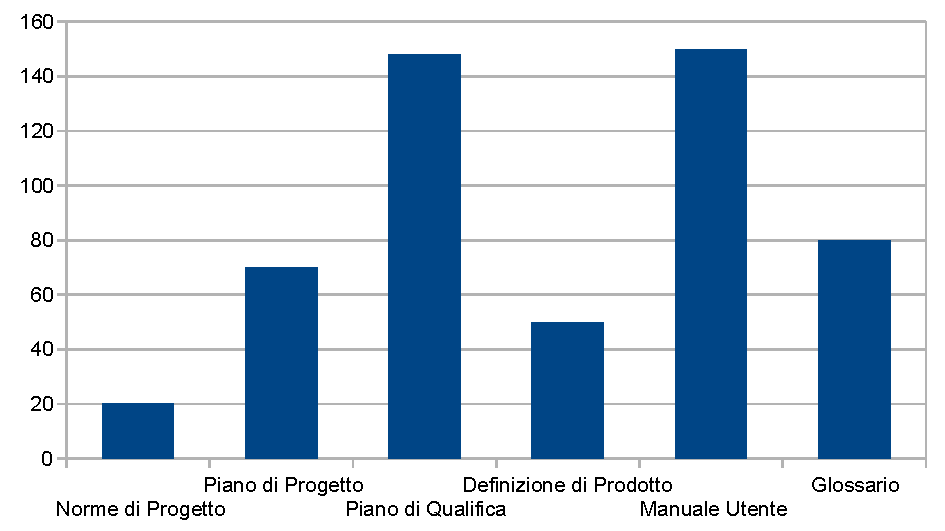
\includegraphics[width=12cm]{PianoDiQualifica/Pics/ProduttivitaDocumentazioneFasePD.pdf}
				\caption{Produttività del processo di documentazione durante la Fase PD}
			\end{figure}

			La produttività media del processo di documentazione è ulteriormente in diminuzione in quanto le nuove sezioni introdotte nei documenti ed eventuali ampliamenti in questa fase sono ridotti al minimo. Ciò contrasta coi livelli di Schedule e Budget Variance a causa del fatto che è stata rivista l'organizzazione dei contenuti dei documenti, non senza sforzo da parte dei membri del Team.

		\level{3}{Processo di verifica}
			\level{4}{Livello CMM}
			In questa fase, il livello del processo di verifica si assesta al terzo gradino della scala CMM, già raggunto nella \insphase{Fase CP}.
			\level{4}{Schedule Variance}
			Il processo di verifica è stato sempre svolto rispettando le scadenze temporali previste nel \insdoc{Piano di Progettov7.00}. I valori della Schedule Variance, calcolati per questo processo, risultano, quindi, ottimi.\\
			Riportiamo di seguito i valori ottenuti:
			\begin{table}[H]
				\centering
				\begin{tabu}{| l | c | c |}
					\hline
						Processi 			& Schedule Variance	& Esito		\\ \hline \hline
						Processo di verifica & 0\% & Ottimale \\ \hline
				\end{tabu}
				\caption{Esiti del calcolo della Schedule Variance durante la Fase PD}
			\end{table}	

			\level{4}{Budget Variance}
			Le risorse utilizzate nel processo di verifica sono di poco maggiori rispetto a quelle preventivate, a causa della necessità di correggere gli errori rilevati nella Revisione di Qualifica. Ciò ha causato un valore accettabile della Budget Variance.
			Riportiamo di seguito il valore ottenuto:
			\begin{table}[H]
				\centering
				\begin{tabu}{| l | c | c |}
				\hline
				Processi 			& Budget Variance	& Esito		\\ \hline \hline
				Processo di verifica & -2\% & Accettabile \\ \hline
				\end{tabu}
				\caption{Esiti del calcolo della Budget Variance durante la Fase PD}
			\end{table}	

			\level{4}{Produttività}
			Utilizzando la formula descritta all'interno del presente documento (sezione \nameref{sec:metriche}) è stata calcolata la produttività del processo di verifica. Tale indice è stato calcolato in seguito a tutti i momenti di verifica previsti dal \insdoc{Piano di Progettov7.00} per la \insphase{Fase PD}. Di seguito vengono riportati i valori calcolati e una loro rappresentazione grafica.
			\begin{table}[H]
				\centering
				\begin{tabu}{| c | c |}
					\hline
					Data verifica & Produttività\\ \hline \hline
					01-02/06 & 3 \\ \hline
					03-05/06 & 10 \\ \hline
					06-11/06 & 16\\ \hline
					11-16/06 & 5\\ \hline
					\end{tabu}
				\caption{Produttività del processo di verifica durante la fase PD}
			\end{table}


			\begin{figure}[H]
				\centering
				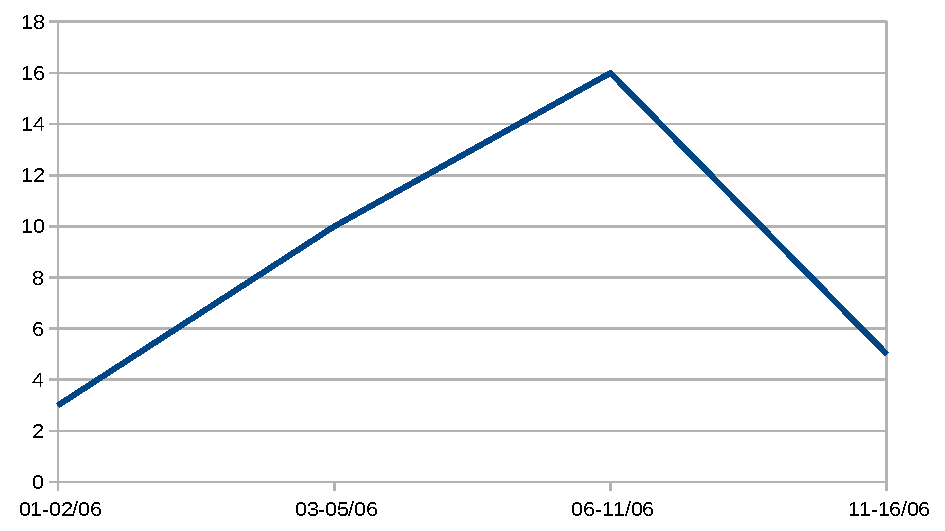
\includegraphics[width=12cm]{PianoDiQualifica/Pics/ProduttivitaVerificaFasePD.pdf}
				\caption{Produttività del processo di verifica durante la Fase PD}
			\end{figure}

			La produttività ha avuto un picco finale dovuto alla necessità di rivedere i documenti presentati alla Revisione di Qualifica, in seguito alle valutazioni ricevute in quel periodo, e alla necessità di verificare il codice prodotto. Si può notare che il livello di produttività è, in media, minore rispetto alle fasi precedenti, questo è dovuto, sempre, al fatto che sono state apportate meno modifiche ai documenti rispetto alle fasi precedenti.

			\level{4}{Efficacia di una revisione}
			Utilizzando la formula descritta all'interno del presente documento (sezione \nameref{sec:metriche}) è stata calcolata l'efficacia delle varie revisioni che sono state fatte durante la \insphase{Fase PD}. Di seguito vengono riportati i valori calcolati ed una loro rappresentazione grafica.
			\begin{table}[H]
				\centering
				\begin{tabu}{| c | c |}
					\hline
						Data verifica & Efficacia\\ \hline \hline
						01-02/06 & 6 \\ \hline
						03-05/06 & 10 \\ \hline
						06-11/06 & 18 \\ \hline
						12-16/06 & 8 \\ \hline
					\end{tabu}
				\caption{Efficacia delle revisioni durante la fase PD}
			\end{table}

			\begin{figure}[H]
				\centering
				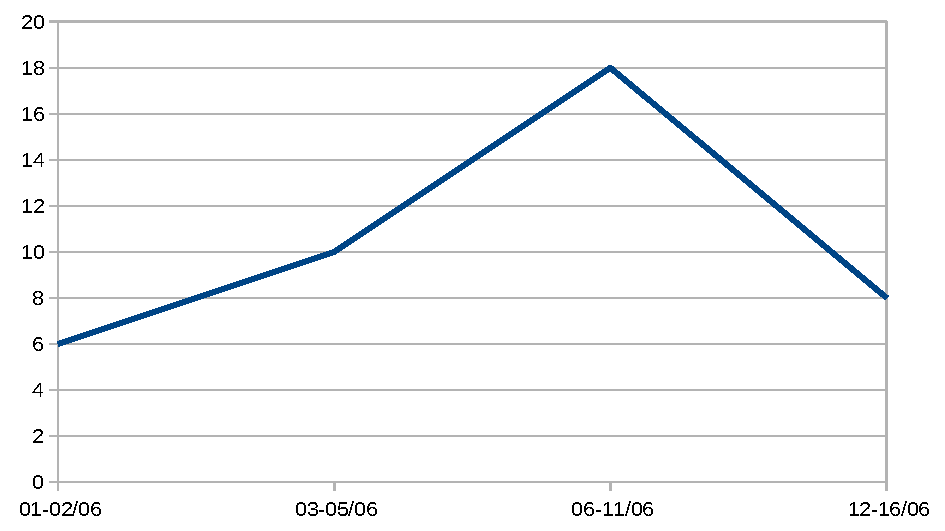
\includegraphics[width=12cm]{PianoDiQualifica/Pics/EfficaciaRevisioniFasePD.pdf}
				\caption{Efficacia delle revisioni durante la Fase PD}
			\end{figure}

			I livelli di efficacia di revisione, nel complesso, rispecchiano l'andamento della produttività. In generale, si ha una bassa efficacia, dovuta ad un basso numero di errori rilevati nei documenti ai quali sono state apportate modifiche. Vi è un picco nel momento in cui sono state apportate modifiche in seguito alle valutazioni ricevute dopo la Revisione di Qualifica.

		\level{3}{Processo di sviluppo}
		Si riportano, in questa sezione, gli esiti delle misurazioni effettuate rispetto all'attività di codifica. In questa fase l'attività di codifica ha avuto un ruolo secondario, in quanto effettuata solo a scopo correttivo.
			\level{4}{Livello CMM}
			Poichè l'attività di codifica è stata attuata solo marginalmente, il livello \insglo{CMM} si attesta sul terzo gradino, raggiunto precedentemente.
			
			\level{4}{Schedule Variance}
			 Riportiamo di seguito i valori ottenuti calcolando la Schedule Variance sui tempi di correzione del codice sorgente.
			\begin{table}[H]
				\centering
				\begin{tabu}{| l | c | c |}
					\hline
						Processi 						& Schedule Variance	& Esito		\\ \hline \hline
						Processo di sviluppo (codifica) & 0\% & Ottimale \\ \hline
				\end{tabu}
				\caption{Esiti del calcolo della Schedule Variance durante la Fase PD}
			\end{table}	
						
			\level{4}{Budget Variance}
			La correzione degli errori sul codice non ha richiesto un particolare dispendio di risorse. Si riporta di seguito il valore della Budget Variance determinato.		\\
			\begin{table}[H]
			\centering
				\begin{tabu}{| l | c | c |}
					\hline
						Processi 						& Budget Variance	& Esito		\\ \hline \hline
						Processo di sviluppo (codifica) & 2\% & Ottimale \\ \hline
				\end{tabu}
				\caption{Esiti del calcolo della Budget Variance dell'attività di codifica durante la Fase PD}
			\end{table}	
							
			\level{4}{Produttività}
			Utilizzando la formula descritta all'interno del presente documento (sezione \nameref{sec:metriche}) è stata calcolata la produttività del processo di sviluppo, limitatamente all'attività di codifica. \\
			Seguono i risultati delle misurazioni.
			\\ 
			\begin{table}[H]
				\centering
				\begin{tabu}{| l | c | c |}
					\hline
						Processi 						& Produttività		\\ \hline \hline
						Processo di sviluppo (codifica) & 46   \\ \hline
				\end{tabu}
				\caption{Esiti del calcolo della produttività della codifica durante la Fase PD}
			\end{table}	
			
		\level{3}{Processo di validazione}
		Si riportano, in questa sezione, gli esiti delle misurazioni effettuate sul processo di Validazione, implementato per ultimo, prima della consegna del prodotto.
			\level{4}{Livello CMM}
			Poichè questo processo è stato attuato per ultimo e per un brevissimo periodo, il team di sviluppo ritiene di aver raggiunto il secondo livello CMM, visto che il processo è stato documentato, ma non sente di aver ancora acquisito una sufficiente padronanza del processo stesso.
			
			\level{4}{Schedule Variance}
			 Riportiamo di seguito i valori ottenuti calcolando la Schedule Variance sulle attività di validazione.
			\begin{table}[H]
				\centering
				\begin{tabu}{| l | c | c |}
					\hline
						Processi 						& Schedule Variance	& Esito		\\ \hline \hline
						Processo di validazione & 0\% & Ottimale \\ \hline
				\end{tabu}
				\caption{Esiti del calcolo della Schedule Variance durante la Fase PD}
			\end{table}	
						
			\level{4}{Budget Variance}
			Riportiamo di seguito i valori ottenuti calcolando la Budget Variance sulle attività di validazione.		\\
			\begin{table}[H]
			\centering
				\begin{tabu}{| l | c | c |}
					\hline
						Processi 						& Budget Variance	& Esito		\\ \hline \hline
						Processo di validazione & 1\% & Ottimale \\ \hline
				\end{tabu}
				\caption{Esiti del calcolo della Budget Variance durante la Fase PD}
			\end{table}	
							
			\level{4}{Produttività}
			Utilizzando la formula descritta all'interno del presente documento (sezione \nameref{sec:metriche}) è stata calcolata la produttività del processo di validazione, espressa in percentuale. \\
			Seguono i risultati delle misurazioni.
			\\ 
			\begin{table}[H]
				\centering
				\begin{tabu}{| l | c | c |}
					\hline
						Processi 						& Produttività		\\ \hline \hline
						Processo di validazione & 100\%   \\ \hline
				\end{tabu}
				\caption{Esiti del calcolo della produttività della codifica durante la Fase PD}
			\end{table}		
					
		\level{3}{PDCA}
		In questa sezione viene riportato il grafico PDCA della \insphase{Fase PD}. In ascissa è rappresentato il tempo, in ordinata le attività.

		% \begin{figure}[H]
		% 	\centering
		% 	\includegraphics[width=0.6\textwidth]{PianoDiQualifica/Pics/GraficoPDCAFasePD.png}
		% 	\caption{PDCA Fase PD}
		% \end{figure}

		Si può facilmente notare come la pianificazione non abbia subito grosse modifiche, rispetto a quanto preventivato. Vi è, quindi, un miglioramento, rispetto alla fase precedente, imputabile all'esperienza acquisita da parte del gruppo e ai pochi incrementi e cambiamenti da apportare ai vari documenti.